\section{Program Generation}
\label{sec:related-work-generation}

The generation of artificial programs is a broad field with a wide range of applications. This section categorises the literature of two use cases that are relevant to this thesis: program generation for performance characterisation, and program generation for compiler validation.

\subsection{Performance Characterisation}
\label{subsec:training-with-synthetic-benchmarks}

Benchmark suites serve a wide variety of uses from compiler optimisations to hardware design. The challenge in creating a benchmark suite is to create a diverse set of workloads that is both representative of the target real world use while providing an adequate coverage of the program space. Achieving either of these two goals is a challenging task, and efforts towards one goal can hamper the other. As a result there is no ``one size fits all'' benchmark suite.

% Ryoo, J. H., Quirem, S. J., Lebeane, M., Panda, R., Song, S., & John, L. K. (2015). GPGPU Benchmark Suites: How Well Do They Sample the Performance Spectrum? ICPP.
An evaluation of GPGPU benchmark suites reveals there are important parts of the program space were left untested~\cite{Ryoo2015}.
% Goswami, N., Shankar, R., Joshi, M., & Li, T. (2010). Exploring GPGPU workloads: Characterization methodology, analysis and microarchitecture evaluation implications. In IISWC. https://doi.org/10.1109/IISWC.2010.5649549
\citeauthor{Goswami2010} evaluate 38 benchmark workloads, finding that \emph{Similarity Score}, \emph{Scan of Large Arrays}, and \emph{Parallel Reduction} workloads show significantly different behaviour due to their large number of diverse kernels, but the remaining 35 workloads provide similar characteristics~\cite{Goswami2010}.
% Xiong, W., Yu, Z., Bei, Z., Zhao, J., Zhang, F., Zou, Y., ... Xu, C. (2013). A Characterization of Big Data Benchmarks. In Big Data. IEEE. https://doi.org/10.1109/BigData.2013.6691707
\citeauthor{Xiong2013} demonstrate that workload behaviour is highly input dependent, and argue that benchmarks created for academic research cannot represent the cases of real world applications~\cite{Xiong2013}.
% Ferdman, M., Adileh, A., Kocberber, O., Volos, S., Alisafaee, M., Jevdjic, D., ... Falsafi, B. (2012). Clearing the Clouds: A Study of Emerging Scale-out Workloads on Modern Hardware. In ASPLOS. ACM.
A review of big data benchmarks found many to be unrepresentative, and that current hardware designs, while optimized for existing benchmark suites, are inefficient for true workloads~\cite{Ferdman2012}.

As well as covering the program space, benchmarks within suites should be diverse.
% Ould-Ahmed-Vall, E., Doshi, K. A., Yount, C., & Woodlee, J. (2008). Characterization of SPEC CPU2006 and SPEC OMP2001: Regression models and their transferability. In ISPASS. IEEE. https://doi.org/10.1109/ISPASS.2008.4510750
\citeauthor{Ould-Ahmed-Vall2008} show that statistical models trained on 10\% of SPEC CPU 2006 data is transferable to the remaining data~\cite{Ould-Ahmed-Vall2008}.
% Phansalkar, A., Joshi, A., & John, L. K. (2007). Analysis of redundancy and application balance in the SPEC CPU2006 benchmark suite. ACM SIGARCH Computer Architecture News, 35(2).
\citeauthor{Phansalkar2007} show that a subset of 14 SPEC CPU 2006 programs can yield most of the information of the entire suite~\cite{Phansalkar2007}, and
% Panda, R., Song, S., Dean, J., & John, L. K. (2018). Wait of a Decade: Did SPEC CPU 2017 Broaden the Performance Horizon? In HPCA. IEEE.
\citeauthor{Draft2018} find that SPEC CPU 2017 contains workloads that can be safely removed without degrading coverage of the program space~\cite{Draft2018}.

Researchers have turned to \emph{synthetic} benchmarks to address the coverage and diversity challenges.
% Curnow, H. J., & Wichmann, B. A. (1976). A Syntetic Benchmark. Computer, 19(1).
The use of synthetic benchmarks is not new, with an early example from \citeyear{Curnow1976} being used to evaluate the compute power of processors for scientific workloads~\cite{Curnow1976}.
% Bell, R. H., & John, L. K. (2005). Improved automatic testcase synthesis for performance model validation. In SC. https://doi.org/10.1145/1088149.1088164
\citeauthor{Bell2005} pose the \emph{synthesis} of synthetic benchmarks as a test case generation problem, using hardware counters to validate the similarity of synthesized benchmarks to a target workload~\cite{Bell2005}.

% Joshi, A. M., Eeckhout, L., Johnz, L. K., & Isen, C. (2008). Automated microprocessor stressmark generation. In HPCA.
A popular use of synthetic benchmark generation techniques is to aid microprocessor design. \citeauthor{Joshi2008} use micro-architecture-independent characteristics such as basic block sizes and data footprint to summarize workloads. Their benchmark generator, \emph{BenchMaker}, then generates a linear sequence of basic blocks and randomly populates them with assembly instructions to match the desired workload characteristics~\cite{Joshi2008}.
% Bertran, R., Buyuktosunoglu, A., Gupta, M. S., Gonzalez, M., & Bose, P. (2012). Systematic Energy Characterization of CMP/SMT Processor Systems via Automated Micro-Benchmarks. In MICRO. IEEE.
\emph{MicroProbe} uses feedback-directed micro-benchmark generation to perform a systematic energy characterisation of an processor~\cite{Bertran2012}.

\emph{GENESIS}~\cite{Chiu2015} is a language for generating synthetic training programs. The essence of the approach is to construct a probabilistic grammar with embedded semantic actions that defines a language of possible programs. New programs may be created by sampling the grammar and, through setting probabilities on the grammar productions, the sampling is biased towards producing programs from one part of the space or another. This technique is potentially completely general, since a grammar can theoretically be constructed to match any desired program domain. However, despite being theoretically possible, it is not easy to construct grammars which are both suitably general and also produce programs that are in any way similar to human written programs. It has been shown to be successful over a highly restricted space of stencil benchmarks with little control flow or program variability~\cite{Garvey2015b,Falch2015,Cummins2015}. But, it is not clear how much effort it will take, or even if it is possible for human experts to define grammars capable of producing human like programs in more complex domains.

Interesting recent developments in synthetic benchmarking have combined elements from feedback-directed test case synthesis (reviewed in the next section) with synthetic benchmarking for the purpose of generating \emph{adversarial} benchmarks that expose performance issues in systems.
% Dhok, M., & Ramanathan, M. K. (2016). Directed Test Generation to Detect Loop Inefficiencies. In FSE. ACM.
\citeauthor{Dhok2016} apply mutation techniques to an initial set of coverage-driven inputs to expose inefficiencies in loops~\cite{Dhok2016}.
% Petsios, T., Zhao, J., Keromytis, A. D., & Jana, S. (2017). SlowFuzz: Automated Domain-Independent Detection of Algorithmic Complexity Vulnerabilities. In CCS. ACM.
\emph{SlowFuzz} uses a resource-usage-guided evolutionary search to find inputs that expose poor algorithmic complexity that could be exploited by attackers to produce Denial-of-Service attacks~\cite{Petsios2017}. It considers the input to a program as a byte sequence and performs mutations to find the byte sequence within a fixed input size that maximizes slowdown.
% Wei, J., Chen, J., Feng, Y., Ferles, K., & Dillig, I. (2018). Singularity: Pattern Fuzzing for Worst Case Complexity. In ESEC/FSE. ACM.
\emph{Singularity} uses an evolutionary search over the space of input \emph{patterns} to find the input with worst case performance~\cite{Wei2018}.
% Toffola, L. D., Pradel, M., & Gross, T. R. (2018). Synthesizing programs that expose performance bottlenecks. In CGO.
\emph{PerfSyn} tackles the related problem of exposing performance bottlenecks from API usage. For a method under test, it starts with a minimal example input and applies a sequence of mutations that modify the original code~\cite{Toffola2018}.
% Lemieux, C., Padhye, R., Sen, K., & Song, D. (2018). PerfFuzz: Automatically Generating Pathological inputs. In ISSTA. ACM. https://doi.org/10.1145/3213846.3213874
\emph{PerfFuzz} uses feedback-directed program mutation to generate programs which maximise execution counts at program locations~\cite{Lemieux2018}.
% Pedrosa, L., Iyer, R., Zaostrovnykh, A., Fietz, J., & Argyraki, K. (2018). Automated Synthesis of Adversarial Workloads for Network Functions. In SIGCOMM. ACM. https://doi.org/10.1145/3230543.3230573
\citeauthor{Pedrosa2018} applies the adversarial benchmark approach to network functions. Their tool, \emph{CASTAN}, takes as input the code for a network function and outputs packet sequences that trigger slow execution paths~\cite{Pedrosa2018}.

In contrast to prior works, the benchmark generation technique proposed in this thesis provides \emph{general-purpose} program generation over unknown domains, in which the statistical distribution of generated programs is automatically inferred from a corpus of real world code. To the best of my knowledge, no prior work has tackled the problem of undirected benchmark generation from example code, as presented in this thesis.


\subsection{Compiler Validation}

Compilers are a fundamental trusted technology, and their correctness is critical. Errors in compilers can introduce security vulnerabilities and catastrophic runtime failures. Therefore, verifying the behaviour of a compiler is of utmost importance.

The complexity of optimizing compilers and programming languages renders formal verification of the entire compiler prohibitively expensive. Efforts have been made in this direction, for example CompCert~\cite{Leroy2013}, a formally verified compiler for the C programming language, but this comes at the cost of supporting only a subset of the language features and with lower performance compared to GCC. Still, even CompCert is not fully verified, and errors have been discovered in the unverified components of it~\cite{Yang2011}.

Because of the difficulties of \emph{verification}, compilers developers turn to \emph{validation}, in which the behaviour of a compiler is validated using a set of input programs, or \emph{test cases}. For each test case, the expected outcome (determined by the specification of the compiler) is compared against the observed outcome to verify that the compiler conforms to the specification, for those inputs. However, the absence of errors for does not prove that the compiler is free from errors unless all possible inputs are tested exhaustively, and the input space for compilers is huge. As such, hand designed suites of test programs, while important, are inadequate for covering such a large space and will not touch all parts of the compiler.

The random generation of programs to test compilers is a well established approach to the compiler validation problem. The main question of interest is in how to efficiently generate codes which trigger bugs. There are two main approaches: \emph{program generation}, where inputs are synthesised from scratch; and \emph{program mutation}, where existing codes are modified so as to identify anomalous behaviour.


\subsubsection{Test Case Generation for Compilers}

The idea of generating test cases for compilers is well established. The majority of test case generation approaches are based on a formal specification of the programming language syntax and grammar.
% Hanford, K. V. (1970). Automatic Generation of Test Cases. IBM Systems Journal, 9(4).
An early approach is presented by \citeauthor{Hanford1970a}, which randomly enumerates a grammar to produce an inexhaustible supply of new programs. While the generated programs are syntactically valid, they are meaningless, and cannot be executed. This limits their value only to testing the compiler front end~\cite{Hanford1970a}.

Deeper testing of compiler components is enabled by generating both a syntactically correct program and a \emph{gold standard output} that would be produced by a conforment compiler. The compiled program can then be executed and its output compared against this gold standard. Figure~\ref{fig:test-case-generators-oracle} shows the process. The challenge of this approach is in generating the gold standard output. These early approaches are surveyed by \citeauthor{Boujarwah1997}~\cite{Boujarwah1997} and \citeauthor{Kossatchev2005}~\cite{Kossatchev2005}.

\begin{figure}
  \centering
  \subfloat[][Expected outcome-based test case generation and evaluation]{%
    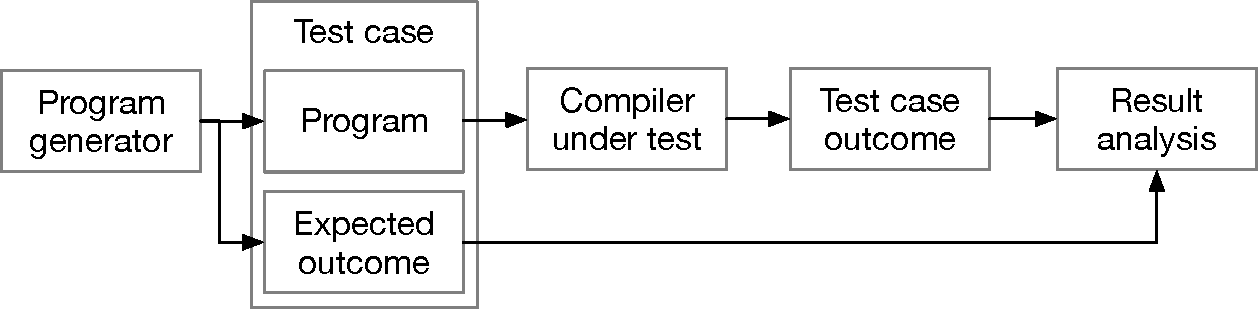
\includegraphics[width=.8\columnwidth]{img/oracle-generator}%
    \label{fig:test-case-generators-oracle}%
  }%
  \\*
  \subfloat[][Differential test case generation and evaluation]{%
    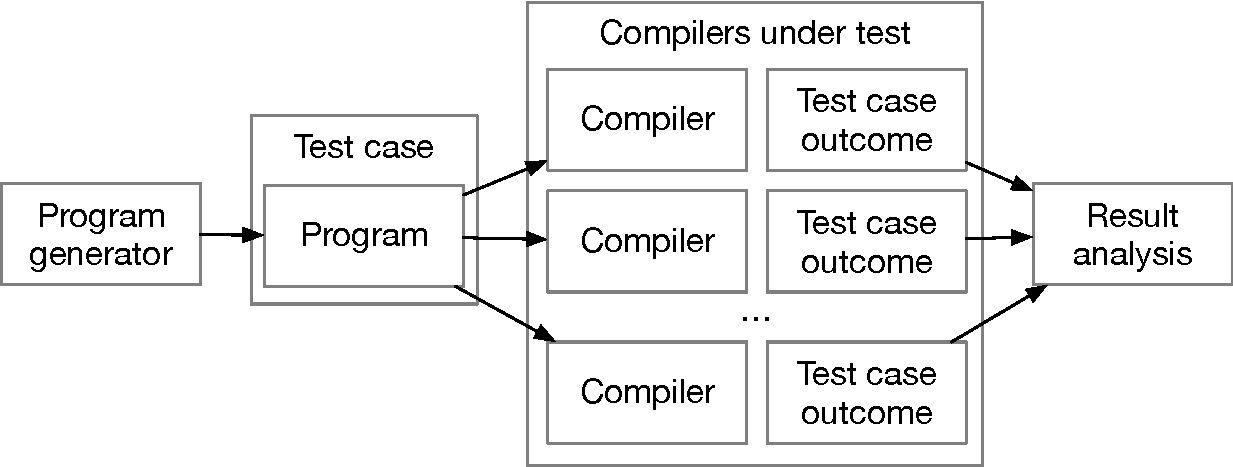
\includegraphics[width=.8\columnwidth]{img/difftest-generator}%
    \label{fig:test-case-generators-difftest}%
  }%
  \caption[Generating and evaluating compiler test cases]{%
    Two approaches to addressing the \emph{compiler validation} problem through test case generation. In~\protect\subref{fig:test-case-generators-oracle}, a test case comprises a program and its expected outcome. In~\protect\subref{fig:test-case-generators-difftest}, only a program is required, and the expected outcome is determined by majority voting on the observed outcomes across multiple compilers.%
  }%
  \label{fig:test-case-generators}
\end{figure}

Differential testing, illustrated in Figure~\ref{fig:test-case-generators-difftest}, accelerates testing by enabling many compilers to be tested at once. The advantage of differential testing over prior approaches is that it does not require a gold standard for the expected behaviour of a conformant compiler. As such, any well formed program may be used as a test. Even malformed inputs may be used to identify anomalies in the error handling logic of compilers. Lacking a gold standard for behaviour makes differential testing less sound than an oracle approach, though in practise the likelihood of the majority consensus being incorrect is extremely unlikely, and no work in the literature has reported such issues. Differential testing can be done across compilers, or using the same compiler with optimizations on or off (or a combination of the two). \citeauthor{Chen2014a} empirically contrasts the two methodologies in~\cite{Chen2014a}, along with a comparison to Equivalence Module Inputs (described in the next subsection).

% McKeeman, W. M. (1998). Differential Testing for Software. DTJ, 10(1).
In the foundational work on differential testing for compilers, McKeeman \emph{et al.\ }present generators capable of enumerating programs of a range of qualities, from random ASCII sequences to C model conforming programs~\cite{McKeeman1998}. Subsequent works have presented increasingly complex generators which improve in some metric of interest, generally expressiveness or probability of correctness.

% Yang, X., Chen, Y., Eide, E., & Regehr, J. (2011). Finding and Understanding Bugs in C Compilers. In PLDI. https://doi.org/10.1145/2345156.1993532
CSmith~\cite{Yang2011} is a widely known and effective generator which enumerates programs by pairing infrequently combined language features. In doing so, it produces correct programs with clearly defined behaviour but very unlikely functionality, increasing the chances of triggering a bug. Achieving this required extensive engineering work, most of it not portable across languages, and ignoring some language features.
% Lidbury, C., Lascu, A., Chong, N., & Donaldson, A. (2015). Many-Core Compiler Fuzzing. In PLDI.
\citeauthor{Lidbury2015a} extend CSmith to the OpenCL programming language, a superficially simple task, yet this required 8 man-months of development and 8000 lines of code~\cite{Lidbury2015a}.
% Nagai, E., Hashimoto, A., & Ishiura, N. (2013). Scaling up Size and Number of Expressions in Random Testing of Arithmetic Optimization of C Compilers. In SASIMI.
Subsequent generators influenced by CSmith, like Orange3~\cite{Nagai2013}, focus on features and bug types beyond the scope of CSmith, arithmetic bugs in the case of Orange3.

% Bastani, O., Sharma, R., Aiken, A., & Liang, P. (2017). Synthesizing Program Input Grammars. In PLDI. https://doi.org/10.1145/3062341.3062349
Glade~\cite{Bastani2017} derives a grammar from a corpus of example programs. The derived grammar is enumerated to produce new programs, though no distribution is learned over the grammar; program enumeration is uniformly random.

Programs generated by grammar-based approaches are often unlike real handwritten code, and are typically very large. As such, once a bug has been identified, test case reduction~\cite{Regehr2012a} is required to minimise the size of the program and isolate the code of interest. Automated test case reduction does not scale to the rate at which effective compilers find bug; sometimes taking hours for a single test case. An alternate method to generating test cases is to instead mutate a seed input.


\subsubsection{Mutation and Feedback-directed Testing}

% Le, V., Afshari, M., & Su, Z. (2014). Compiler Validation via Equivalence Modulo Inputs. In PLDI. https://doi.org/10.1145/2594291.2594334
Equivalence Modulo Inputs (EMI) testing, introduced by~\citeauthor{Le2013a}~\cite{Le2013a} follows a different approach to test case generation. Starting with existing code, it inserts or deletes statements that will not be executed so that the functionality of the code is unchanged. If it is affected, it is due to a compiler bug. \emph{Hermes} extends the initial EMI approach to permit the mutation of \emph{live code} regions, not just dead code~\cite{Sun2016a}. This greatly increases the expressiveness of the generated programs.

\emph{LangFuzz} also uses program mutation but does this by inserting code segments which have previously exposed bugs. This increases the chances of discovering vulnerabilities in scripting language engines~\cite{Holler2012}.
% Peng, H., Shoshitaishvili, Y., & Payer, M. (2018). T-Fuzz: Fuzzing by Program Transformation. In SP.
Starting with a coverage-guided set of inputs, \emph{T-Fuzz} uses dynamic tracing to detect input checks in programs and selectively removes them to expose defects~\cite{Peng2018}.
% Zhang, Q., Sun, C., & Su, Z. (2017). Skeletal Program Enumeration for Rigorous Compiler Testing. In PLDI.
\emph{Skeletal program enumeration} again works by transforming existing code. It identifies algorithmic patterns in short pieces of code and enumerates all the possible permutations of variable usage~\cite{Zhang2017a}.
% Mathis, B., Kampmann, A., Gopinath, R., Höschele, M., Mera, M., & Zeller, A. (2019). Parser-Directed Fuzzing. In PLDI.
\emph{pFuzzer} targets input parsers, using dynamic tainting to produce a set of legal inputs that cover all conditions during parsing~\cite{Mathis2019}.
% Chen, Y., Su, T., Sun, C., Su, Z., & Zhao, J. (2016). Coverage-Directed Differential Testing of JVM Implementations. In PLDI.
Coverage-directed mutation techniques have been for differential testing the Java Virtual Machine~\cite{Chen2016b}.

Machine learning has been used to guide test case mutation.
% Cheng, L., Zhang, Y., Zhang, Y., Wu, C., Li, Z., Fu, Y., & Li, H. (2019). Optimizing seed inputs in fuzzing with machine learning. ArXiv:1902.02538.
\citeauthor{Cheng2019} construct neural networks to discover correlation between PDF test case and execution in the target program. The correlations are then leveraged to generate new paths in the target program~\cite{Cheng2019}.
% She, D., Pei, K., Epstein, D., Yang, J., Ray, B., & Jana, S. (2018). NEUZZ: Efficient Fuzzing with Neural Program Learning. ArXiv:1807.05620.
\emph{NEUZZ} learns a differentiable neural approximation of target program logic, then uses Stochastic Gradient Descent to guide program mutation~\cite{She2018}.
% Wang, J., Chen, B., Wei, L., & Liu, Y. (2017). Skyfire: Data-Driven Seed Generation for Fuzzing. In S&P. https://doi.org/10.1109/SP.2017.23
\emph{Skyfire} learns a probabilistic context-sensitive grammar over a corpus of programs to generate input seeds for mutation testing~\cite{Wang2017c}. The generated seeds are shown to improve the code coverage of AFL~\cite{Zalewski} when fuzzing XSLT and XML engines. The seeds are not directly used as test cases.

EMI and feedback-directed approaches rely on having a large number of seed programs to mutate. As such, it often still requires an external code generator. Similarly to CSmith, these methods tend to favour very long test programs.


\subsubsection{Neural Program Generation}

Recently, machine learning methods have been proposed for generating test cases. These differ from prior works that use machine learning to guide the generation of test cases.
% Jozefowicz, R., Vinyals, O., Schuster, M., Shazeer, N., & Wu, Y. (2016). Exploring the Limits of Language Modeling. arXiv:1602.02410.
Many methods based are based on the astonishing success of Recurrent Neural Networks (RNNs) at modelling sequential data~\cite{Jozefowicz2016a}. RNNs have been successfully applied to a variety of other generative tasks, including image captioning~\cite{Vinyals}, colourising black and white photographs~\cite{Zhang2016}, artistic style~\cite{Gatys2015}, and image generation~\cite{Gregor2014}.

% Sutskever, I., Vinyals, O., & Le, Q. V. (2014). Sequence to Sequence Learning with Neural Networks. In NIPS.
The proficiency of RNNs for sequence modelling is demonstrated in~\cite{Sutskever2014}. \citeauthor{Sutskever2014} apply two RNN networks to translate first a sequence into a fixed length vector, then to decode the vector into an output sequence. This architecture achieves state-of-the-art performance in machine translation. The authors find that reversing the order of the input sequences markedly improves translation performance by introducing new short term dependencies between input and output sequences.

% Neelakantan, A., Le, Q. V., & Sutskever, I. (2016). Neural Programmer: Inducing Latent Programs with Gradient Descent. In ICLR.
Although nascent, the use of neural networks to generate programs is evolving rapidly. \emph{Neural Programmer} was an early example at program generation through the latent representation of a neural network~\cite{Neelakantan2016}.
% Godefroid, P., Peleg, H., & Singh, R. (2017). Learn&Fuzz: Machine Learning for Input Fuzzing. In ASE.
Most similar to the work presented in this thesis is \emph{Learn\&fuzz}, in which an LSTM network is trained over a corpus of PDF files to generate test inputs for the Microsoft Edge renderer, yielding one bug~\cite{Godefroid2017}. Unlike compiler testing, PDF test cases require no inputs and no pre-processing of the training corpus.
% Liu, X., Li, X., Prajapati, R., & Wu, D. (2019). DeepFuzz: Automatic Generation of Syntax Valid C Programs for Fuzz Testing. In AAAI.
\emph{DeepFuzz} uses a sequence-to-sequence model to generate C programs, uncovering 8 bugs in GCC. Unlike the technique presented in this work, sampling occurs only occurs on white-space so as to maximise the probability of a generated program being syntactically correct, though this does not address the issue of semantic correctness~\cite{Liu2019}.
% Nasrabadi, M. Z., Parsa, S., & Kalaee, A. (2018). Neural Fuzzing: A Neural Approach to Generate Test Data for File Format Fuzzing. ArXiv:1812.09961.
\emph{IUST DeepFuzz} is a neural file generator for file format fuzzing, trained and evaluated on a corpus of PDF files~\cite{Nasrabadi2018}.
% Brockschmidt, M., Allamanis, M., Gaunt, A. L., & Polozov, O. (2018). Generative Code Modeling with Graphs.
\citeauthor{Brockschmidt2018} present a novel methodology for program generation in which a graph is used as the intermediate representation~\cite{Brockschmidt2018}.

Machine learning has been used for other purposes in testing other than program generation, reviewed in Section~\ref{sec:related-work-other}.
